\documentclass[article]{jss}
\usepackage[utf8]{inputenc}

\author{
Zhenke Wu\\Johns Hopkins University \And Scott L. Zeger\\Johns Hopkins University
}
\title{\pkg{baker}: Bayesian Analysis Kit for Etiology Research}
\Keywords{Bayesian hierarchical models, latent variable models, learning health community, measurement error, Markov chain Monte Carlo, individualized health, \proglang{R}, visualization, \proglang{WinBUGS}}

\Abstract{
Clinicians are routinely inferring the differential causes of patients'
diseases, also known as disease etiology, from a set of clinical or
laboratory measurements indicative of the unobserved disease status.
However, such diagnoses are usually based on judgement and experience of
individual doctors. As the measurements become complex in diagnostic
evidence and large in volume, doctors would benefit from principled
methods to integrate and extract signals from various predictive
measurements, to compare the effectiveness of available treatment
alternatives and to optimize ensuing treatment algorithms. In this
article, we describe a methodological framework, known as the ``learning
health community'' for considering general problems involving latent
disease status and treatment effect evaluations. We illustrate the
framework with a hierarchical Bayesian model to infer disease etiology
for multivariate binary data using a new R package \texttt{baker}. The
package builds in functionalists for data cleaning, exploratory data
analyses, model specification, model estimation, visualization and model
diagnostics and comparisons, catalyzing vital effective communications
between analysts and practitioner clinicians. \texttt{baker} has
implemented models for dependent measurements given disease status,
regression analyses of etiology, multiple imperfect measurements,
different priors for true positive rates among cases with differential
measurement characteristics, and multiple-pathogen etiology. The
complete workflow and usage of the package are illustrated by both
simulated and actual data from the motivating Pneumonia Etiology
Research for Child Health (PERCH) study.
}

\Plainauthor{Zhenke Wu, Scott L. Zeger}
\Plaintitle{A Capitalized Title: Something about a Package foo}
\Shorttitle{\pkg{baker}: An R package for Bayesian Analysis of Etiology}
\Plainkeywords{keywords, not capitalized, Java}

%% publication information
%% \Volume{50}
%% \Issue{9}
%% \Month{June}
%% \Year{2012}
\Submitdate{}
%% \Acceptdate{2012-06-04}

\Address{
    Zhenke Wu\\
  Johns Hopkins University\\
  Department of Biostatistics Baltimore, Maryland 21205, U.S.A.\\
  E-mail: \href{mailto:zhwu@jhu.edu}{\nolinkurl{zhwu@jhu.edu}}\\
  URL: zhenkewu.com\\~\\
      Scott L. Zeger\\
  Johns Hopkins University\\
  Department of Biostatistics Baltimore, Maryland 21205, U.S.A.\\
  E-mail: \href{mailto:sz@jhu.edu}{\nolinkurl{sz@jhu.edu}}\\
  
  }

\usepackage{amsmath}

\begin{document}

\section{Introduction}\label{introduction}

We describe and illustrate a statistical framework for individualized
health through a case study of estimating disease childhood pneumonia
etiology (Levine, O'Brien, Deloria-Knoll, et al., 2012).

\section{Models}\label{models}

\subsection{Measurement Models}\label{measurement-models}

We first discuss the partially-latent class models (pLCM) Wu,
Deloria-Knoll, Hammitt, et al. (2015) with conditional independence
assumptions. For a list of latent status (etiologic causes in PERCH), we
have multiple measurements that are collected to infer the distribution
of latent status for the diseased population and latent status for
individual subjects.The measurements are generally of two levels of
quality:

\begin{enumerate}
\def\labelenumi{\arabic{enumi}.}
\itemsep1pt\parskip0pt\parsep0pt
\item
  Bronze-Standard (BrS) data that are available for both cases and
  controls but with imperfect sensitivity or specificity; Each
  measurement is a multivariate binary vector.
\item
  Silver-Standard (SS) data that are only available among cases. It has
  perfect specificity but imperfect sensitivity; Each measurement is a
  multivariate binary vector.
\end{enumerate}

To allow multiple measurements to jointly inform latent status, we use a
template for each measurement pair of (specimen, test) in PERCH, e.g.,
nasal-pharyngeal (NP) swab specimens tested by PCR technology) to
indicate how we connect or ``plug'' measurements to latent status.

The following are example templates for cases from 4 pairs of (specimen,
test): NP PCR, Whole Blood (WB) PCR, NP Culture (CX) and Blood (B)
Culture. Data obtained from the first three are BrS data and the last
one is SS data. One feature of such representation is the measurements
are connected by shared latent status, i.e., every row of each template
table represents a category of latent status that can cause a pneumonia
case. There are many possible extensions of this framework. For example,
if a measurement exists to inform all bacterial latent status, then
bacterial latent status rows will all be ones for that measurement's
template. If more than one sub-populations are concerned, we may have
separate templates, one for each stratum defined by covariates.
Technically, 1s indicate that we need to use true positive rates to
describe the observed measurement on a pathogen for cases caused by the
latent status belonging to that row; 0s indicate that we need to use
false positive rates estimated from control population, whose templates
for these measurements have all zero entries.

\begin{CodeChunk}
\begin{table}

\caption{NPPCR}
\begin{tabular}{l|r|r|r|r|r}
\hline
  & HINF & PNEU & PARA1 & RHINO & RSV\\
\hline
HINF & 1 & 0 & 0 & 0 & 0\\
\hline
PNEUVT13 & 0 & 1 & 0 & 0 & 0\\
\hline
PNEUNOVT13 & 0 & 1 & 0 & 0 & 0\\
\hline
PARA1 & 0 & 0 & 1 & 0 & 0\\
\hline
RHINO & 0 & 0 & 0 & 1 & 0\\
\hline
RSV & 0 & 0 & 0 & 0 & 1\\
\hline
ENTRB & 0 & 0 & 0 & 0 & 0\\
\hline
TB & 0 & 0 & 0 & 0 & 0\\
\hline
HINF+RSV & 1 & 0 & 0 & 0 & 0\\
\hline
ENTRB+TB & 0 & 0 & 0 & 0 & 0\\
\hline
control & 0 & 0 & 0 & 0 & 0\\
\hline
\end{tabular}
\end{table}

\begin{table}

\caption{WBPCR}
\begin{tabular}{l|r}
\hline
  & PNEU\\
\hline
HINF & 0\\
\hline
PNEUVT13 & 1\\
\hline
PNEUNOVT13 & 1\\
\hline
PARA1 & 0\\
\hline
RHINO & 0\\
\hline
RSV & 0\\
\hline
ENTRB & 0\\
\hline
TB & 0\\
\hline
HINF+RSV & 0\\
\hline
ENTRB+TB & 0\\
\hline
control & 0\\
\hline
\end{tabular}
\end{table}

\begin{table}

\caption{NPCX}
\begin{tabular}{l|r|r}
\hline
  & PNEUVT13 & PNEUNOVT13\\
\hline
HINF & 0 & 0\\
\hline
PNEUVT13 & 1 & 0\\
\hline
PNEUNOVT13 & 0 & 1\\
\hline
PARA1 & 0 & 0\\
\hline
RHINO & 0 & 0\\
\hline
RSV & 0 & 0\\
\hline
ENTRB & 0 & 0\\
\hline
TB & 0 & 0\\
\hline
HINF+RSV & 0 & 0\\
\hline
ENTRB+TB & 0 & 0\\
\hline
control & 0 & 0\\
\hline
\end{tabular}
\end{table}

\begin{table}

\caption{BCX}
\begin{tabular}{l|r|r|r|r|r}
\hline
  & HINF & PNEUVT13 & PNEUNOVT13 & ENTRB & TB\\
\hline
HINF & 1 & 0 & 0 & 0 & 0\\
\hline
PNEUVT13 & 0 & 1 & 0 & 0 & 0\\
\hline
PNEUNOVT13 & 0 & 0 & 1 & 0 & 0\\
\hline
PARA1 & 0 & 0 & 0 & 0 & 0\\
\hline
RHINO & 0 & 0 & 0 & 0 & 0\\
\hline
RSV & 0 & 0 & 0 & 0 & 0\\
\hline
ENTRB & 0 & 0 & 0 & 1 & 0\\
\hline
TB & 0 & 0 & 0 & 0 & 1\\
\hline
HINF+RSV & 1 & 0 & 0 & 0 & 0\\
\hline
ENTRB+TB & 0 & 0 & 0 & 1 & 0\\
\hline
control & 0 & 0 & 0 & 0 & 0\\
\hline
\end{tabular}
\end{table}

\end{CodeChunk}

These templates describe for every dimension of a measurement (every
column) the positive rates. To describe the joint probability of a
vector of measurements (all columns), conditional independence model
assumes that the measurements are not informative of one another given
the knowledge of a case's disease status (i.e., which row a case
belongs).

\subsection{Priors}\label{priors}

There are three sets of priors used in the model.

For conditional independence model (pLCM):

\begin{quote}
\begin{itemize}
\itemsep1pt\parskip0pt\parsep0pt
\item
  True positive rate (\(\mathbf{\Theta}\))

  \begin{itemize}
  \itemsep1pt\parskip0pt\parsep0pt
  \item
    Bronze-standard (BrS) data; set by function
    \texttt{set\_prior\_tpr\_BrS()}
  \item
    Silver-standard (SS) data; \texttt{set\_prior\_tpr\_SS()}
  \end{itemize}
\item
  False positive rate (\(\mathbf{\Psi}\))

  \begin{itemize}
  \itemsep1pt\parskip0pt\parsep0pt
  \item
    Bronze-standard (BrS) data; non-informative priors
    \texttt{beta(1,1)}
  \end{itemize}
\item
  Etiology pie (\(\mathbf{\pi}\)); set by function
  \texttt{overall\_uniform()}
\end{itemize}
\end{quote}

\subsection{Posterior Computing}\label{posterior-computing}

We use the open-source statistical software R for data preprocessing,
operations and visualization. Another freely available Bayesian
inference software, WinBUGS is used to conduct posterior inference of
all unknown parameters in the model. We use the R package
\texttt{R2WinBUGS} to connect R and WinBUGS for streamlined analyses.
The results will be generated and stored in a specified directory, which
contains necessary information (e.g., posterior samples of unknown
parameters, data, priors, likelihood specifications) for posterior
analyses included in the \texttt{baker} package.

\section{Software Components}\label{software-components}

There are six functional components altogether forming a analysis
pipeline:

\begin{enumerate}
\def\labelenumi{\arabic{enumi}.}
\itemsep1pt\parskip0pt\parsep0pt
\item
  Clean/Prepare data
\item
  Exploratory data analysis (EDA)
\item
  Specify model
\item
  Fit model
\item
  Check model
\item
  Visualize results
\end{enumerate}

We illustrate the workflow by the following conceptual figure:

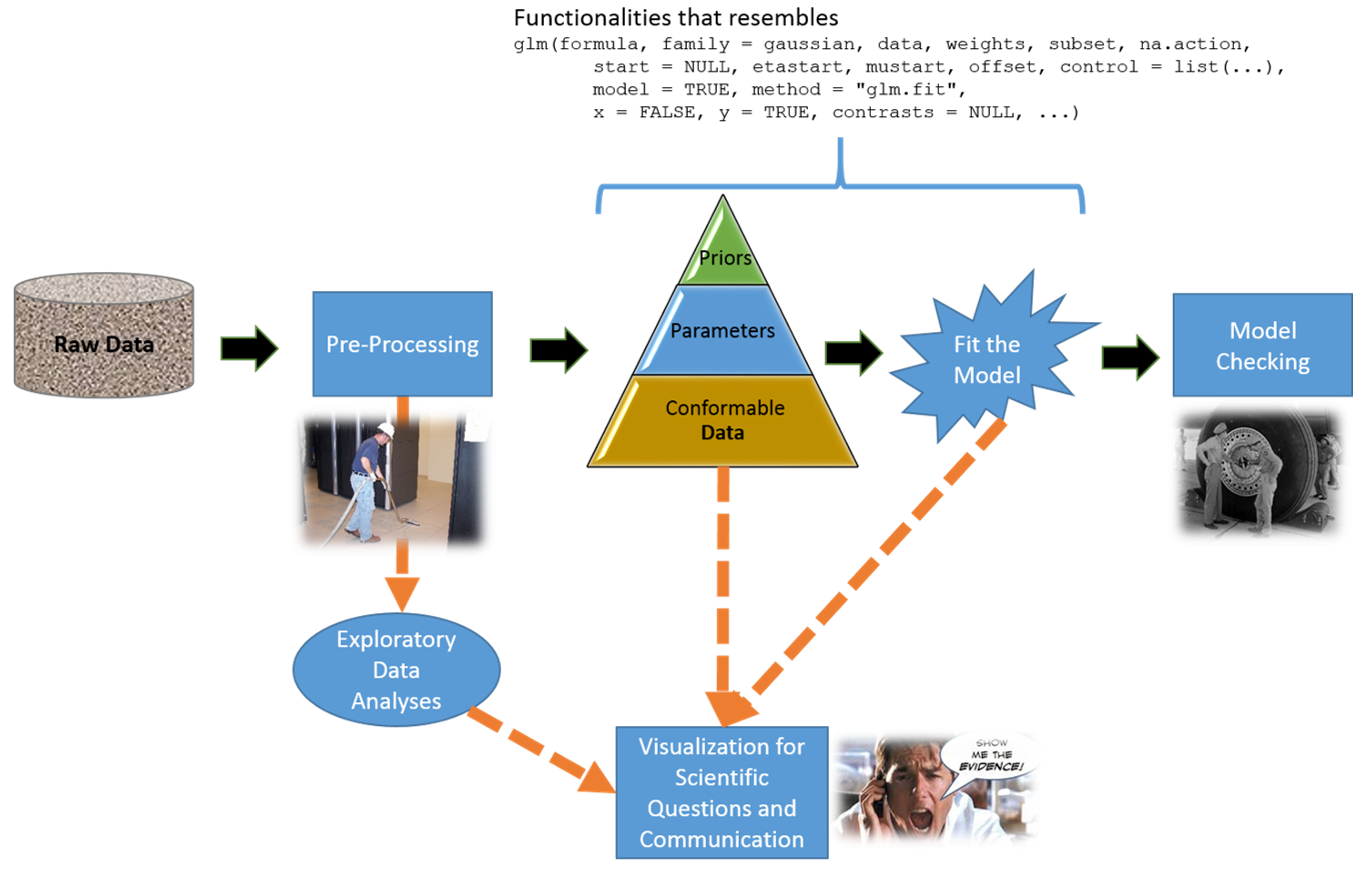
\includegraphics{./figures/software_structure_illustration.png}

In the following, we collect variable and function definitions using
terms that are motivated by PERCH study to provide an easy and
scientifically grounded interface for analysts. We will convert them to
generic names in future versions of \texttt{baker}, because the model is
a general discrete state model. We put relevant file structures in
shaded paragraphs.

\subsection{Raw Data}\label{raw-data}

\subsubsection{PERCH Data}\label{perch-data}

We start by describing ingredients in PERCH raw data. In the data table,
the rows are for subjects, and columns stores information on
case-control status, lab measurements, as well as other epidemiological
or demographic covariates such as age, HIV status, enrollment date, etc.

The software \texttt{baker} is designed to infer latent variables
(unobserved lung infections in PERCH) from the complex lab measurements.
The lab measurements are named as
\texttt{{[}PATHOGEN\ NAME{]}\_{[}SPECIMEN\ NAME{]}{[}ASSAY\ NAME{]}}.
For example, the column \texttt{PNEU\_NPPCR} represents the polymerase
chain reaction (PCR) measurements for the bacteria \emph{Streptococcus
pneumoniae} (PNEU) using specimen from nasal-pharyngeal (NP) swabs. The
results are coded as pathogen presence (1) or absence (0).

We also have taxonomy information about the studied pathogens that tells
us which ones are bacteria, viruses, or sub-serotypes nested within a
species (e.g., PNEU has many serotypes).

\subsection{Clean Data}\label{clean-data}

We first preprocess the raw PERCH data into a form that is analyzable by
\texttt{baker}.

\subsubsection{PERCH Data}\label{perch-data-1}

We collect lab measurements, case-control status and other covariates
into \texttt{data\_nplcm}:

\begin{enumerate}
\def\labelenumi{\arabic{enumi}.}
\itemsep1pt\parskip0pt\parsep0pt
\item
  \texttt{Mobs}: A list of measurements. The elements of the list should
  include MBS, MSS, and MGS. If any of the component is not available,
  please specify it as, e.g., MGS=NULL (effectively deleting MGS from
  Mobs).

  \begin{itemize}
  \itemsep1pt\parskip0pt\parsep0pt
  \item
    \texttt{MBS}: a list of data frames of bronze-standard (BrS)
    measurements. Each element of the list has its name being the
    (specimen, test) pair. In each element (a data frame), rows are
    subjects, columns are pathogens with column names being pathogens.
    They have imperfect sensitivity/specificity (e.g.~nasal-pharyngeal
    PCR).
  \item
    \texttt{MSS}: a list of data frames of silver-standard (SS)
    measurements. Rows are subjects, columns are pathogens measured in
    specimen (e.g.~blood culture). These measurements have perfect
    specificity but imperfect sensitivity.
  \item
    \texttt{MGS}: a list of data frames of gold-standard (GS)
    measurements. Rows are subject, columns are pathogen measurements.
    These measurements have perfect sensitivity and specificity.
  \end{itemize}
\item
  \texttt{Y}: Vector of disease status: 1 for case, 0 for control.
\item
  \texttt{X}: A data frame of covariates for regression modeling. It
  contains raw covariate data specified by \texttt{X\_strat} and
  \texttt{X\_extra}. It is not design matrix for regression models.
\end{enumerate}

This is the structure of the most basic data type for the model. There
are functions in \texttt{baker} that would require information that is
not data, e.g., the template to refer each measurement to the category
of latent status that is useful in model fitting.

This structure is automatically generated as outputs from both
functions: \texttt{clean\_perch\_data()} and \texttt{simuate\_nplcm()}.

\begin{quote}
\begin{itemize}
\itemsep1pt\parskip0pt\parsep0pt
\item
  \texttt{clean\_perch\_data()}

  \begin{itemize}
  \itemsep1pt\parskip0pt\parsep0pt
  \item
    \texttt{clean\_combine\_subsites()}
  \item
    \texttt{extract\_data\_raw()}
  \item
    \texttt{make\_meas\_object()}
  \item
    \texttt{show\_individual()}
  \end{itemize}
\end{itemize}
\end{quote}

\subsubsection{Simulated Data}\label{simulated-data}

We will use simulated data (cleaned by definition) to demonstrate
functions for visualization, analysis, data summary as well as to
facilitate comparisons with other methods, such as population
attributable fractions.

To simulate data sets in the framework of npLCM, we need to specify the
following parameters: population etiology pie \(\mathbf{\pi}\), true
positive rates \(\mathbf{\Theta}\), false positive rates
\(\mathbf{\Psi}\).

\begin{quote}
\begin{itemize}
\itemsep1pt\parskip0pt\parsep0pt
\item
  \texttt{simulate\_nplcm()} for simulating measurement data without
  knowing actual latent status of observations;

  \begin{itemize}
  \itemsep1pt\parskip0pt\parsep0pt
  \item
    \texttt{simulate\_latent()} samples latent status for each subject;
  \item
    \texttt{simulate\_brs()} samples bronze-standard measurements based
    on sampled latent status;
  \item
    we can add extra measurements by writing functions similar to
    \texttt{simulate\_ss()}, say to generate silver-standard
    measurements.
  \end{itemize}
\end{itemize}
\end{quote}

\subsection{Exploratory Data Analysis
(EDA)}\label{exploratory-data-analysis-eda}

Model-free display of raw data information.

\begin{quote}
\begin{itemize}
\itemsep1pt\parskip0pt\parsep0pt
\item
  \texttt{plot\_logORmat()}: plot pairwise log odds ratios along with
  standardized estimate and t-statistic for cases and controls.
\end{itemize}
\end{quote}

\subsection{Specify Model}\label{specify-model}

The \texttt{baker} package can fit multiple models with various
specifications of measurement likelihood and prior. The main workhorse
of this package is a high-level \texttt{nplcm()} which can interpret the
model specifications and call low-level model fitting functions for the
analyses introduced in the next section.

We allow the user to specify which model to fit along with prior
information through \texttt{model\_options} which contains
\texttt{likelihood}, \texttt{use\_measurements} and \texttt{prior}.

\begin{quote}
\begin{enumerate}
\def\labelenumi{\arabic{enumi}.}
\itemsep1pt\parskip0pt\parsep0pt
\item
  \textbf{\texttt{likelihood}}

  \begin{itemize}
  \itemsep1pt\parskip0pt\parsep0pt
  \item
    \texttt{cause\_list} The vector of latent status;
  \item
    \texttt{k\_subclass} The number of nested subclasses. 1 for
    conditional independence, \textgreater{}1 for conditional
    dependence;
  \item
    \texttt{Eti\_formula} formula for etiology regressions. You can use
    dm\_Rdate\_Eti to specify the design matrix for R format enrollment
    date; it will produce natural cubic splines for every date. Specify
    \textasciitilde{}0 if no regression is intended.
  \item
    \texttt{FPR\_formula} formula for false positive rates (FPR)
    regressions; see formula. You can use dm\_Rdate\_FPR to specify part
    of the design matrix for R format enrollment date; it will produce
    thin-plate regression spline basis for every date (if
    effect=``random'' and num\_knots\_FPR is specified to a positive
    integer, e.g., 10.). If effect=``fixed'', dm\_Rdate\_FPR will just
    specify a design matrix with appropirately standardized dates.
    Specify \textasciitilde{}0 if no regression is intended.
  \end{itemize}
\item
  \textbf{\texttt{use\_measurements}}

  \begin{itemize}
  \itemsep1pt\parskip0pt\parsep0pt
  \item
    a vector of characters strings; can be any singleton or combinaitons
    of ``BrS'', ``SS'', ``GS''.
  \end{itemize}
\item
  \textbf{\texttt{prior}}

  \begin{itemize}
  \itemsep1pt\parskip0pt\parsep0pt
  \item
    \texttt{Eti\_prior} Description of etiology prior (e.g., one can use
    \texttt{overall\_uniform()} to specify hyperpriors for latent status
    distribution);
  \item
    \texttt{TPR\_prior} Description of priors for the true positive
    rates for measurements. Check illustrative examples for more
    details.
  \end{itemize}
\end{enumerate}
\end{quote}

These parameters are first used by \texttt{assign\_model()} to interpret
the model to fit. It will compare the actual data provided against the
specification. When it detects the data are not conformable to feed in
the user-specified model, \texttt{assign\_model()} will instruct how to
re-prepare data (assuming correct model specification).

\subsection{Fit Model}\label{fit-model}

The fitting function \texttt{nplcm()} takes in the following three
arguments:

\begin{quote}
\begin{itemize}
\itemsep1pt\parskip0pt\parsep0pt
\item
  \texttt{nplcm()}

  \begin{itemize}
  \itemsep1pt\parskip0pt\parsep0pt
  \item
    \texttt{data\_nplcm}
  \item
    \texttt{model\_options}
  \item
    \texttt{mcmc\_options}
  \end{itemize}
\end{itemize}
\end{quote}

The function \texttt{nplcm()} can fit the following models:

\begin{itemize}
\itemsep1pt\parskip0pt\parsep0pt
\item
  No formal regression analysis

  \begin{itemize}
  \itemsep1pt\parskip0pt\parsep0pt
  \item
    measurement conditional independence model: done.
  \item
    measurement conditional \emph{dependence} model
  \end{itemize}
\item
  Regression analysis

  \begin{itemize}
  \itemsep1pt\parskip0pt\parsep0pt
  \item
    measurement conditional independence model
  \item
    measurement conditional \emph{dependence} model
  \end{itemize}
\end{itemize}

Because we currently use WinBUGS for Bayesian inference of the models,
we need to provide \texttt{.bug} files with model likelihood and prior.
The package \texttt{baker} can interpret the specified models and write
them in \texttt{.bug} files. For example, \texttt{baker} uses
\texttt{write\_model\_NoReg\_NoNest()} to write .bug file for models
without regression and conditional independence model, accommodating
multiple bronze-standard (any standard) data and covariate-stratified
(e.g., antibiotic use) TPRs for silver-standard data.

\subsection{Check Model}\label{check-model}

Posterior predictive checking: * \texttt{check\_common\_pattern()} and
\texttt{check\_common\_pattern\_two\_folders()} *
\texttt{check\_pairwise\_logOR()} and
\texttt{check\_pairwise\_logOR\_two\_folders()}

\subsection{Visualize Results}\label{visualize-results}

\texttt{baker} provides powerful tools for visualizing Bayesian
inference results of the distribution of latent status structure for the
population and an individual. The figures are designed to facilitate
easier communications between analysts and domain experts (e.g.,
epidemiologists and clinicians in PERCH study). The plotting functions
assume a model has been fitted with posterior samples and model settings
stored at a folder. The visualization functions and figures produced
from them are listed below.

\begin{itemize}
\item
  \texttt{plot\_group\_etiology()}: density function of two-group
  fraction, for example, the probability of viral etiology. The figure
  also includes cascaded ternary diagrams down the taxonomy, e.g., the
  fractions of the most, second-most frequent viruses and other viruses.

  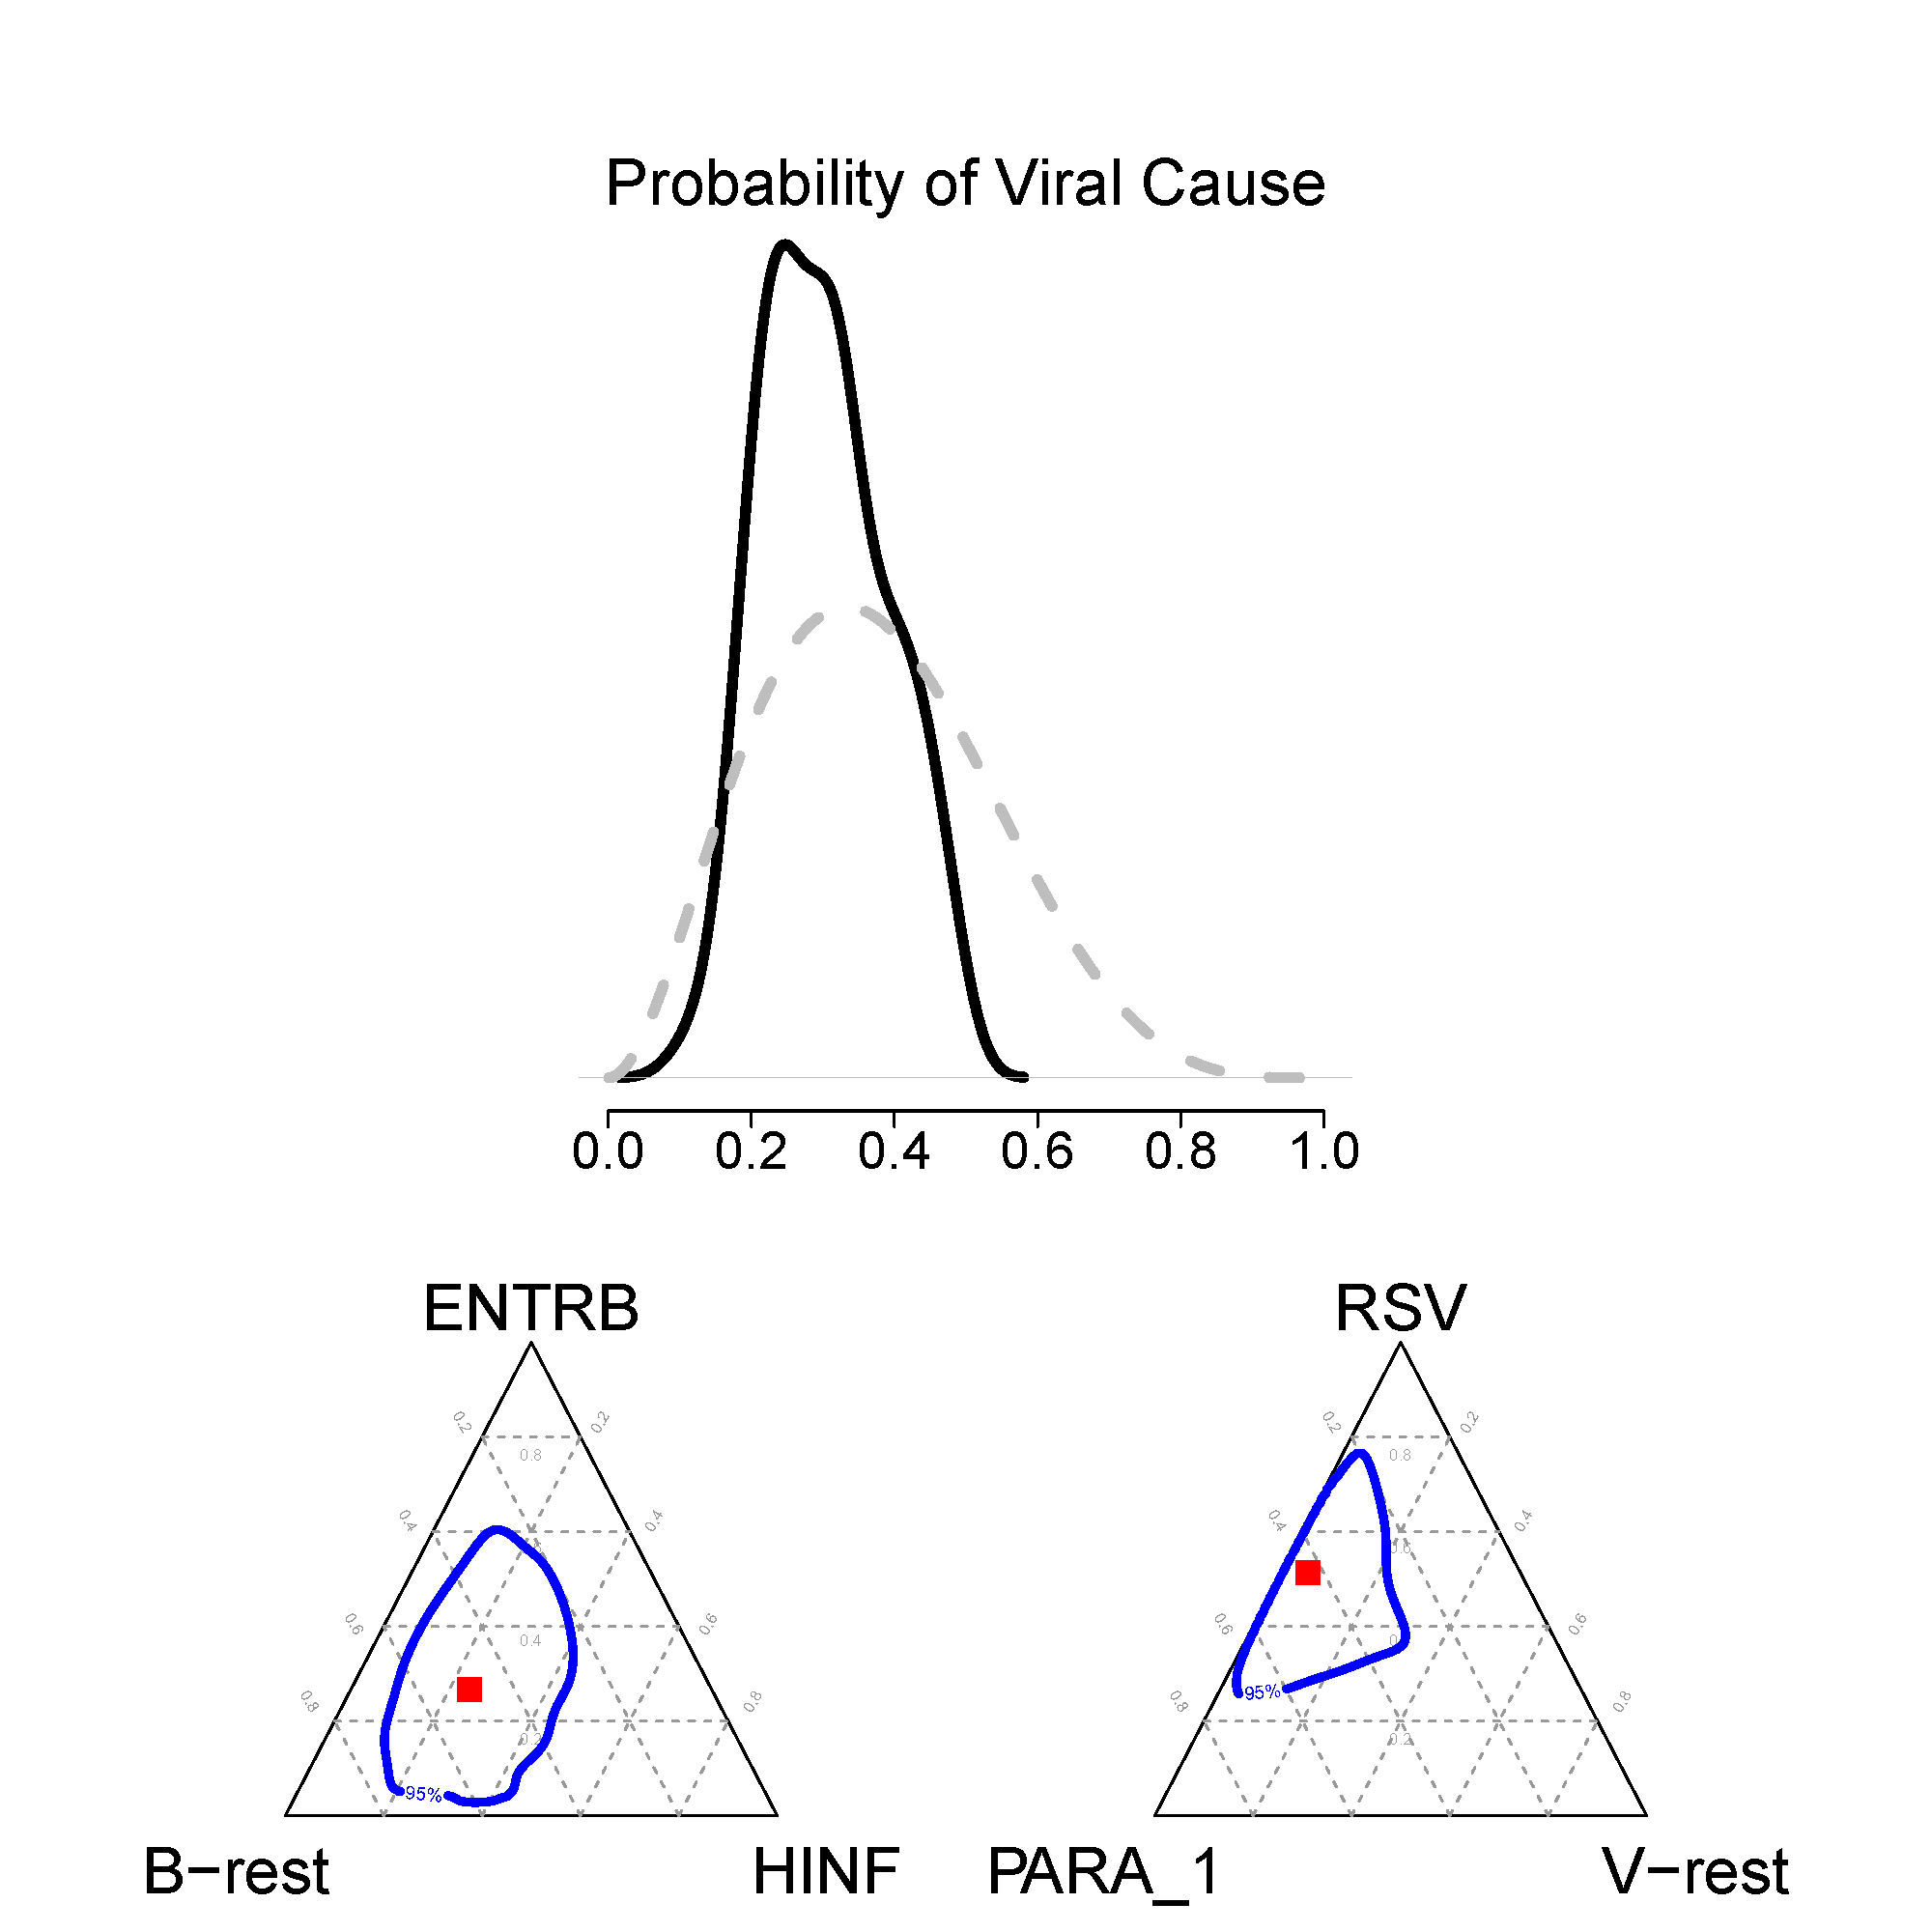
\includegraphics{./figures/grouped_etiology.png}
\item
  \texttt{plot\_selected\_etiology()}: triangle plot for selected three;
\item
  \texttt{plot\_panels()}: a multi-panel figure that puts data, prior
  and posterior together. In our experience, it is most effective for
  research on understanding information for disease etiology and
  measurement characteristics as well as the synergy among all types of
  available measurement data.
\end{itemize}

\begin{CodeChunk}


\begin{center}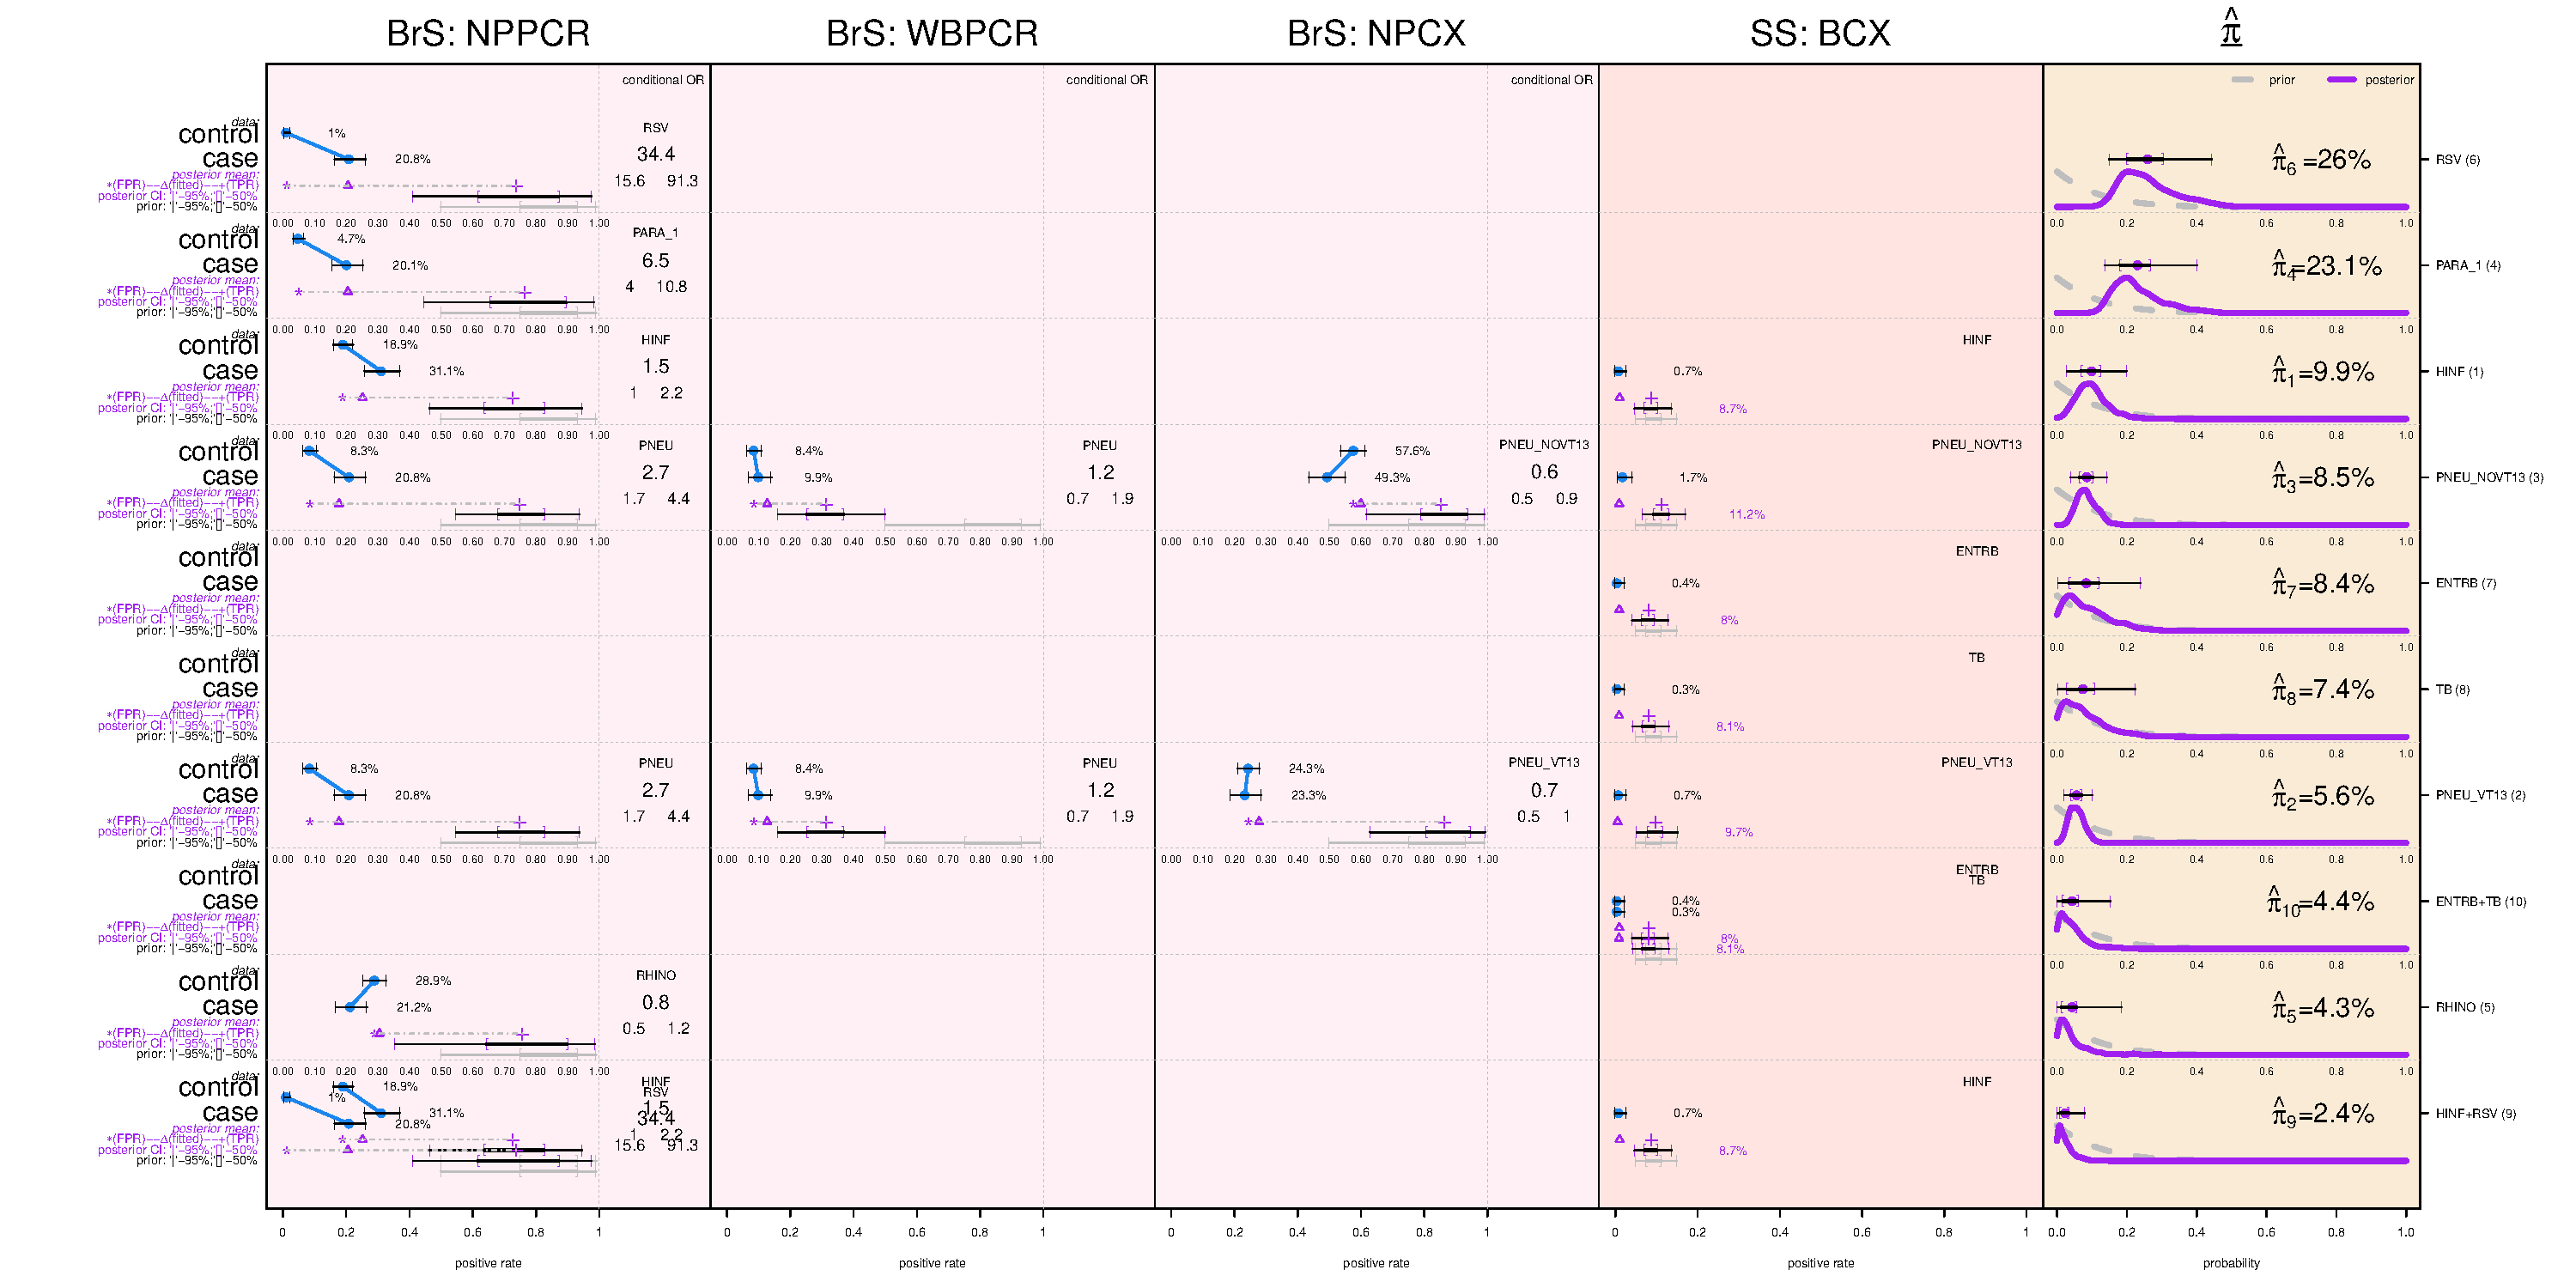
\includegraphics{figures/unnamed-chunk-3-1} \end{center}

\end{CodeChunk}

\begin{itemize}
\itemsep1pt\parskip0pt\parsep0pt
\item
  individual prediction
\end{itemize}

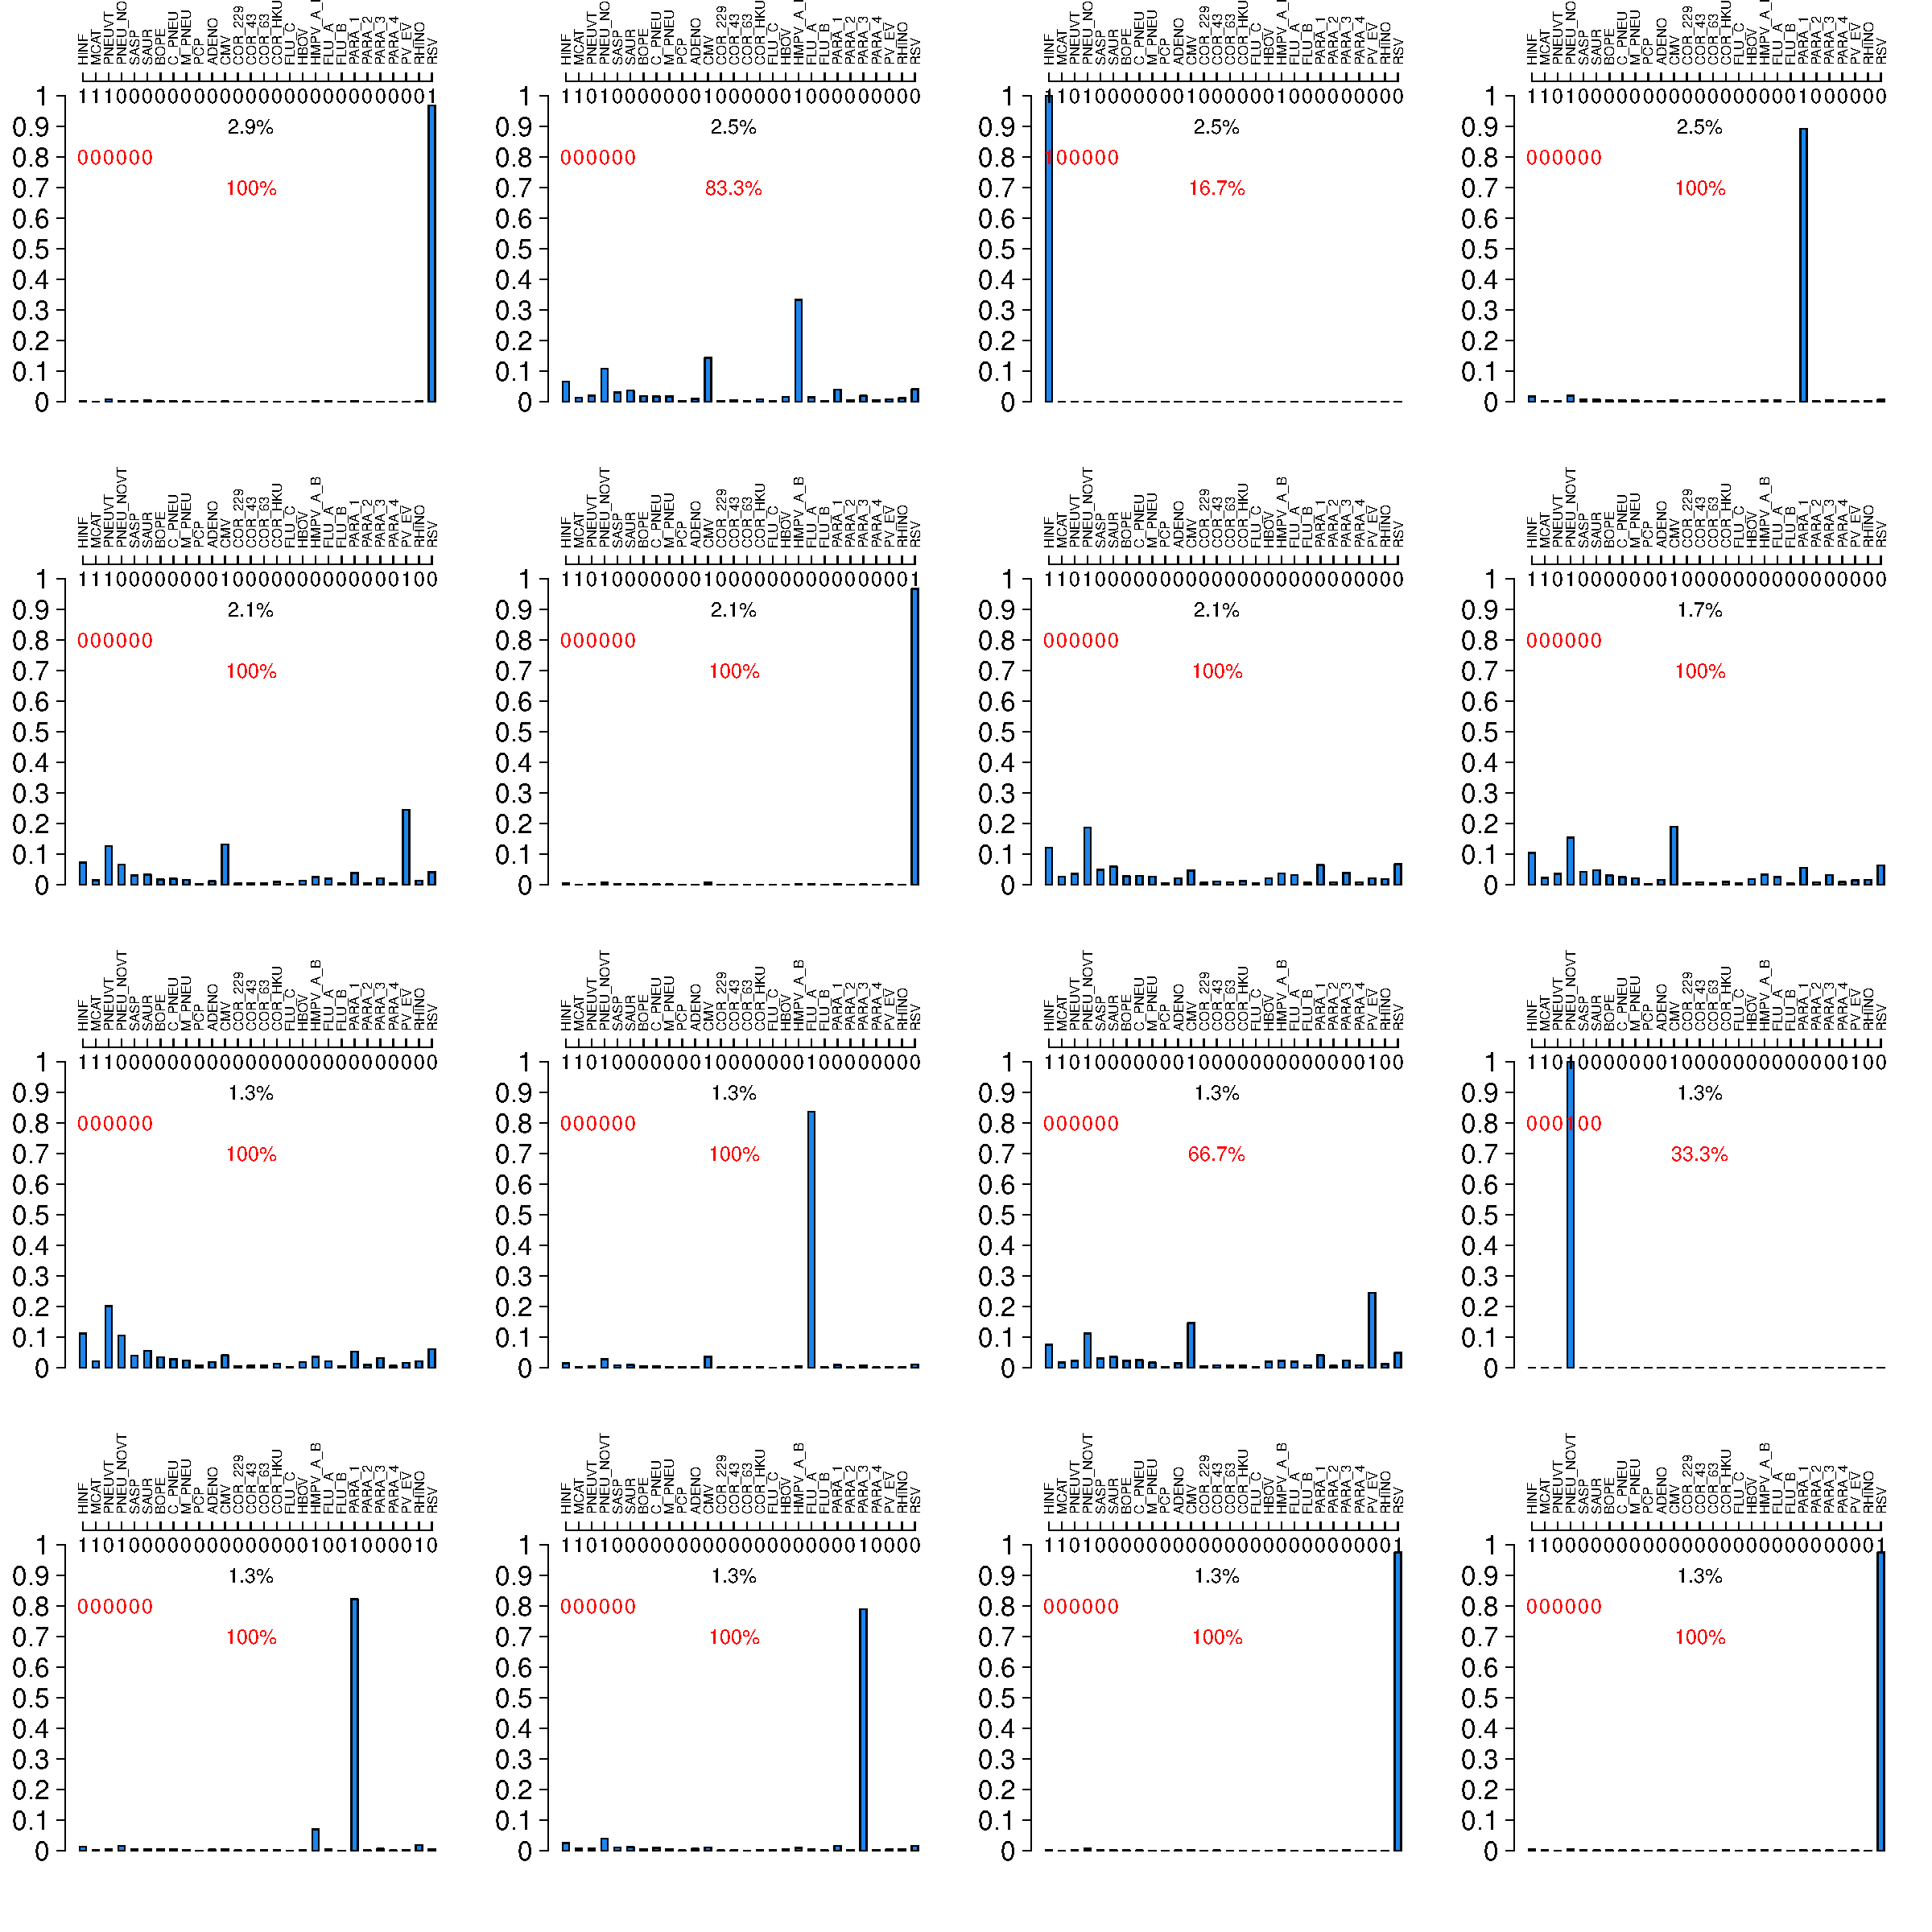
\includegraphics{./figures/02GAM_individual_diagnosis.pdf}

\begin{itemize}
\itemsep1pt\parskip0pt\parsep0pt
\item
  regression visualization
\end{itemize}

\section{Examples}\label{examples}

\subsection{Simulated Examples}\label{simulated-examples}

\subsection{PERCH Study}\label{perch-study}

\section{Discussion}\label{discussion}

\section{Reference}\label{reference}

{[}1{]} O. Levine, K. O'Brien, M. Deloria-Knoll, et al. ``The Pneumonia
Etiology Research for Child Health Project: A 21st Century Childhood
Pneumonia Etiology Study''. In: Clinical Infectious Diseases 54.suppl 2
(2012), pp.~S93--S101.

{[}2{]} Z. Wu, M. Deloria-Knoll, L. L. Hammitt, et al. ``Partially
latent class models for case--control studies of childhood pneumonia
aetiology''. In: Journal of the Royal Statistical Society: Series C
(Applied Statistics) (2015), p.~DOI: 10.1111/rssc.12101.

\end{document}

